\documentclass[a4paper, 10pt]{article}

\usepackage{../packages}

\graphicspath{{./figures/}}

\hypersetup{
	colorlinks=true,
	linkcolor=blue,
	filecolor=magenta,
	urlcolor=cyan,
	pdftitle={Synteza układu wnioskującego},
	pdfpagemode=FullScreen,
}

\begin{document}

\begin{titlepage}
\begin{center}
	
\includegraphics[scale=0.7]{logo.png}

	\vspace*{4cm}
	\textbf{Sztuczna inteligencja\\ Laboratorium}

	\vspace{1.5cm}
	\textit{Synteza układu wnioskującego}

	\vspace{1.5cm}
	\textbf{Stanislau Antanovich}\\
	nr. indeksu: 173590\\
	gr. lab: L04
\end{center}
\end{titlepage}

\tableofcontents
\listoffigures

\newpage

% intro section
\section{Wstęp}\label{sec:wstep}
\subsection{Cel ćwiczenia}\label{subsec:cel}

Laboratorium składa się z trzech zasadniczych części. Część \ref{sec:expert_system} ma na celu zapoznanie się ze sposobem syntezy rozmytego systemu ekspertowego typu Mamdaniego z wykorzystaniem biblioteki \textbf{scikit-fuzzy}. W części \ref{sec:modyfikacja}, należy zapoznać się z ideą działania systemu Mamdaniego a następnie dokonać modyfikacji systemu wykonanego w części \ref{sec:expert_system}. Część \ref{sec:modyfikacja} laboratorium polega na wykonaniu przykładowego zadania zaliczeniowego.

% expert system section
\section{System ekspertowy typu Mamdaniego}\label{sec:expert_system}
\subsection{Problem}\label{subsec:problem}

Zaprojektować rozmyty układ ekspertowy doradzający ile napiwku pozostawić w restauracji na podstawie oceny jakości obsługi oraz jakości jedzenia. Jakość obsługi i jakość jedzenia będzie oceniana w skali od 1 do 10, gdzie 10 reprezentuję ocenę maksymalną, natomiast napiwek będzie liczbą z przedziału [0,30] reprezentującą procent wartości rachunku.

Baza reguł będzie składała się z 5 reguł. System zostanie wykonany w dwóch etapach. W \textbf{etapie pierwszym}(rys. \ref{fig:obsluga} i \ref{fig:napiwek}) system będzie zbudowany z jednego wejścia(\emph{obsługa}) i jednego wyjścia(\emph{napiwek}) oraz 3 reguł postaci:
\begin{itemize}
	\item[R1] \emph{jeżeli obsługa jest słaba, to napiwek jest mały}
	\item[R2] \emph{jeżeli obsługa jest dobra, to napiwek jest średni}
	\item[R3] \emph{jeżeli obsługa jest wspaniała, to napiwek jest duży}
\end{itemize}

\begin{figure}[H]
	\centering
	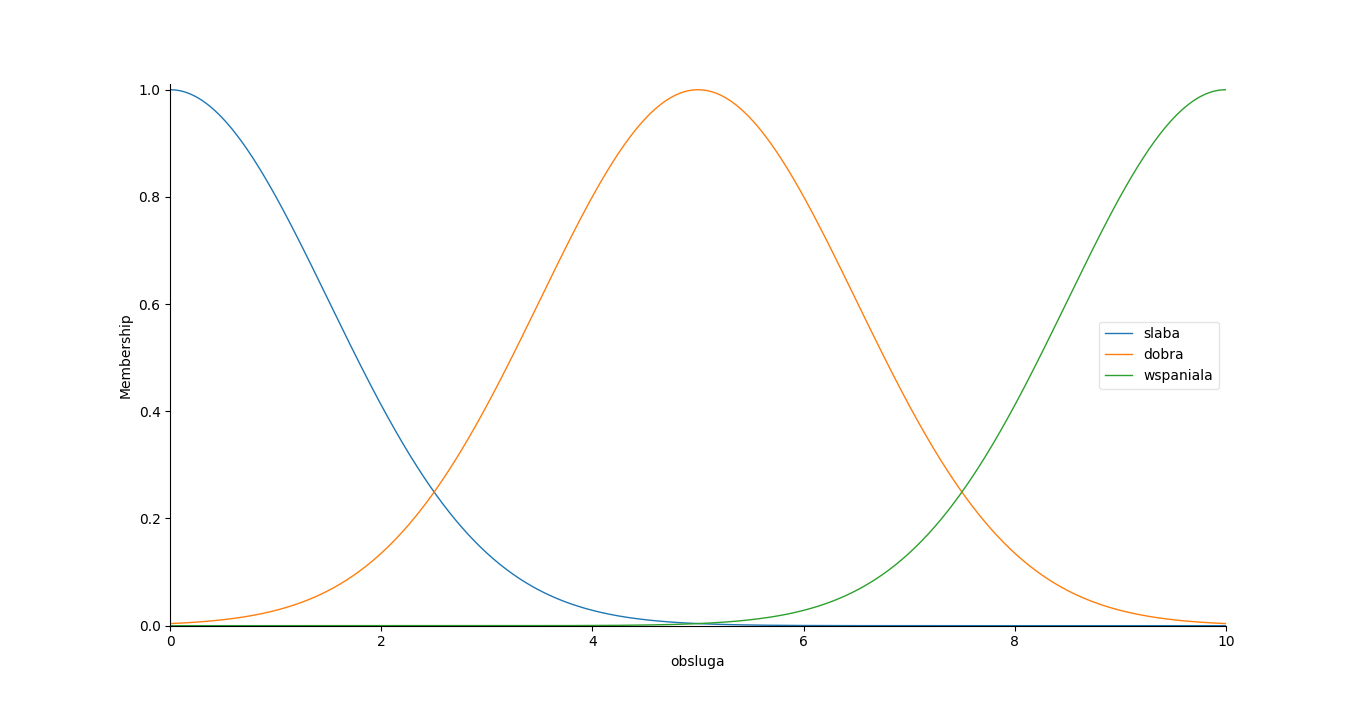
\includegraphics[scale=0.35]{Figure_1.png}
	\caption{\textit{Obsługa}}
	\label{fig:obsluga}
\end{figure}

\begin{figure}[H]
	\centering
	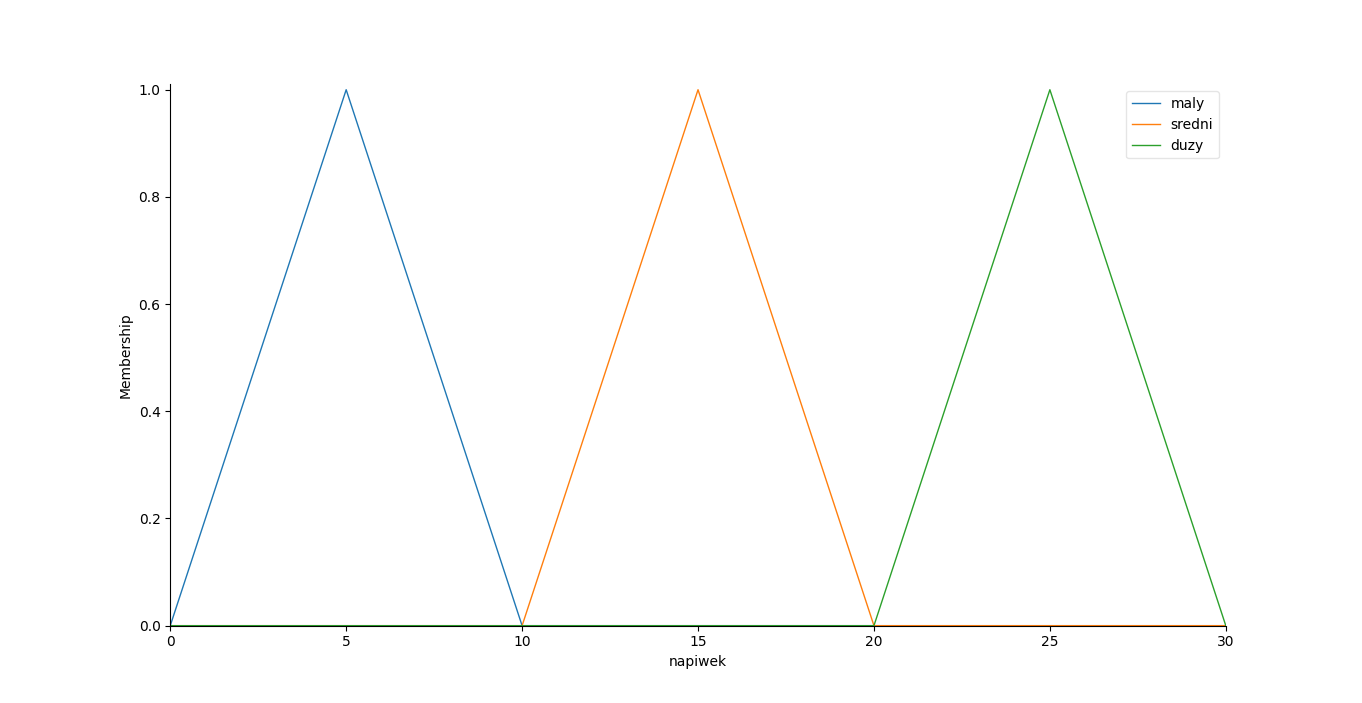
\includegraphics[scale=0.35]{Figure_2.png}
	\caption{\textit{Napiwek}}
	\label{fig:napiwek}
\end{figure}

W \textbf{etapie drugim} do systemu zostanie dodane gruga zmienna wejściowa \emph{jedzenie}(rys. \ref{fig:jedzenie}) oraz 2 dodatkowe reguły
\begin{itemize}
	\item[R4] \emph{jeżeli jedzenie jest zepsute, to napiwek jest mały}
	\item[R5] \emph{jeżeli jedzenie jest wyborne, to napiwek jest duży}
\end{itemize}

\begin{figure}[H]
	\centering
	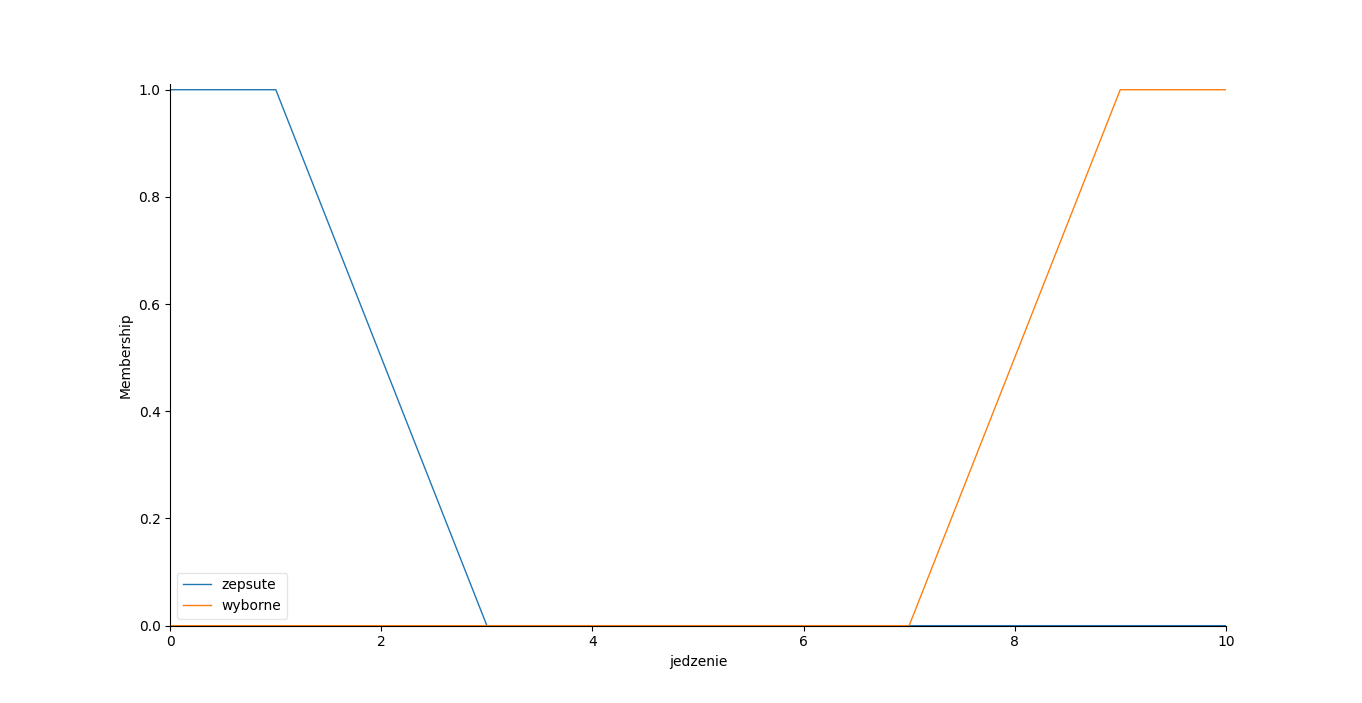
\includegraphics[scale=0.35]{Figure_6.png}
	\caption{\textit{Jedzenie}}
	\label{fig:jedzenie}
\end{figure}

\subsection{Realizacja}\label{subsec:realizacja}
\subsubsection{Inicjowanie modułów}\label{ssc:inicjowanie}

W tej sekcji inicjujemy wszystkie wymagane biblioteki dla prawidłowego działania programu.

\lstinputlisting[firstline=0, lastline=4, style=PYTHON]{./code/main.py}

\subsubsection{Tworzenie zmiennych stanu poprzednika ``obsługa'' oraz następnika ``napiwek''}\label{ssc:tworzenie}

W tej sekcji tworzymy zmienne stanu poprzednika ``obsługa'' oraz następnika ``napiwek''.

\lstinputlisting[style=PYTHON, firstline=6, lastline=7]{./code/main.py}

\subsubsection{Dodanie zbiorów rozmytych}\label{ssc:dodanie_zbiorow_rozmytych}
 
W tej sekcji do zminnej \emph{obsługa} dodajemy następujące zbiory: \emph{slaba, dobra, wspaniala}. 

Zbiór \emph{slaba} o centrum umieszczonym w punkcie uniwersum równym \textbf{0} i rozpiętości wynoszącej \textbf{1.5}. Dla zbiorów \emph{dobra} i \emph{wspaniala} o centrach ulokowanych w punktach odpowiednio \textbf{5} oraz \textbf{10} i rozpiętości wynoszącej \textbf{1.5}

Dla zmiennej \emph{napiwek} dodajemy zbiory trójkątne: \emph{maly, sredni, duzy} o parametrach [0, 5, 10], [10, 15, 20] i [20, 25, 30] odpowiednio.

\lstinputlisting[style=PYTHON, firstline=10, lastline=16]{./code/main.py}

\subsubsection{Podgląd zbiorów rozmytych}\label{ssc:podglad_zbiorow}

Podgląd zbiorów rozmytch można zrealizować metodą \verb|view()| dla poszczególnych zmiennych stanu.

\lstinputlisting[style=PYTHON, firstline=21, lastline=22]{./code/main.py}

\subsubsection{Definicja reguł}\label{ssc:definicja_regul}

W tej sekcji definiujemy reguły.

\lstinputlisting[style=PYTHON, firstline=25, lastline=27]{./code/main.py}

\subsubsection{Dodanie reguł do systemu rozmytego}\label{ssc:dodanie_regul}

W tej sekcji dodajemy powyżej zdefiniowane reguły do systemu rozmytego.

\lstinputlisting[style=PYTHON, firstline=31, lastline=32]{./code/main.py}

\subsubsection{Sprawdzenie działania systemu}\label{ssc:sprawdzenie_dzialania}

W tej sekcji sprawdzamy działanie systemu dla wartości obsługi równej \textbf{0}(rys. \ref{fig:obsluga0}) oraz dla wartości równej \textbf{10}(rys. \ref{fig:obsluga10}).

\lstinputlisting[style=PYTHON, firstline=35,lastline=39]{./code/main.py}

Wartość napiwku dla wartości obsługi wynosi: 5.07657801

Wartość napiwku dla wartości obsługi wynosi: 24.9234219

\begin{figure}[H]
	\centering
	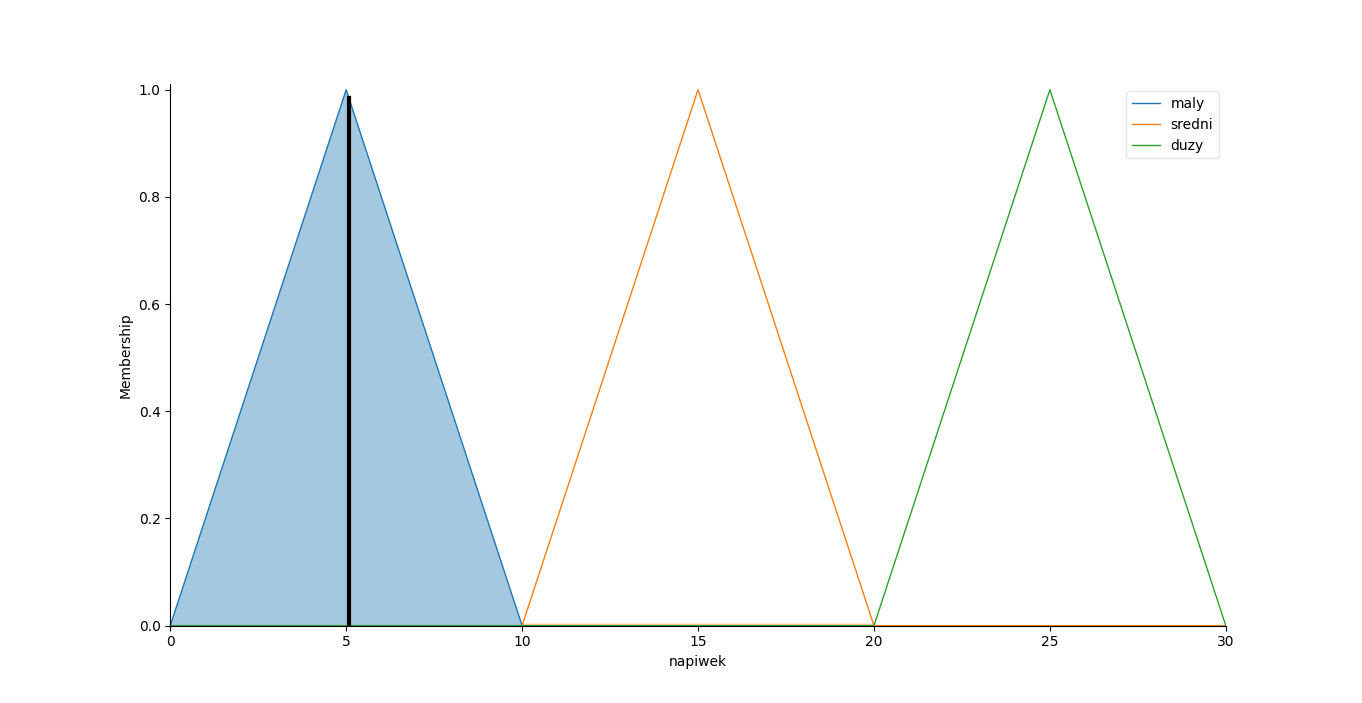
\includegraphics[scale=0.35]{Figure_3.png}
	\caption{\textit{Wyostrzenie metodą środka ciężkości dla wejścia obsługa = 0}}
	\label{fig:obsluga0}
\end{figure}

\begin{figure}[H]
	\centering
	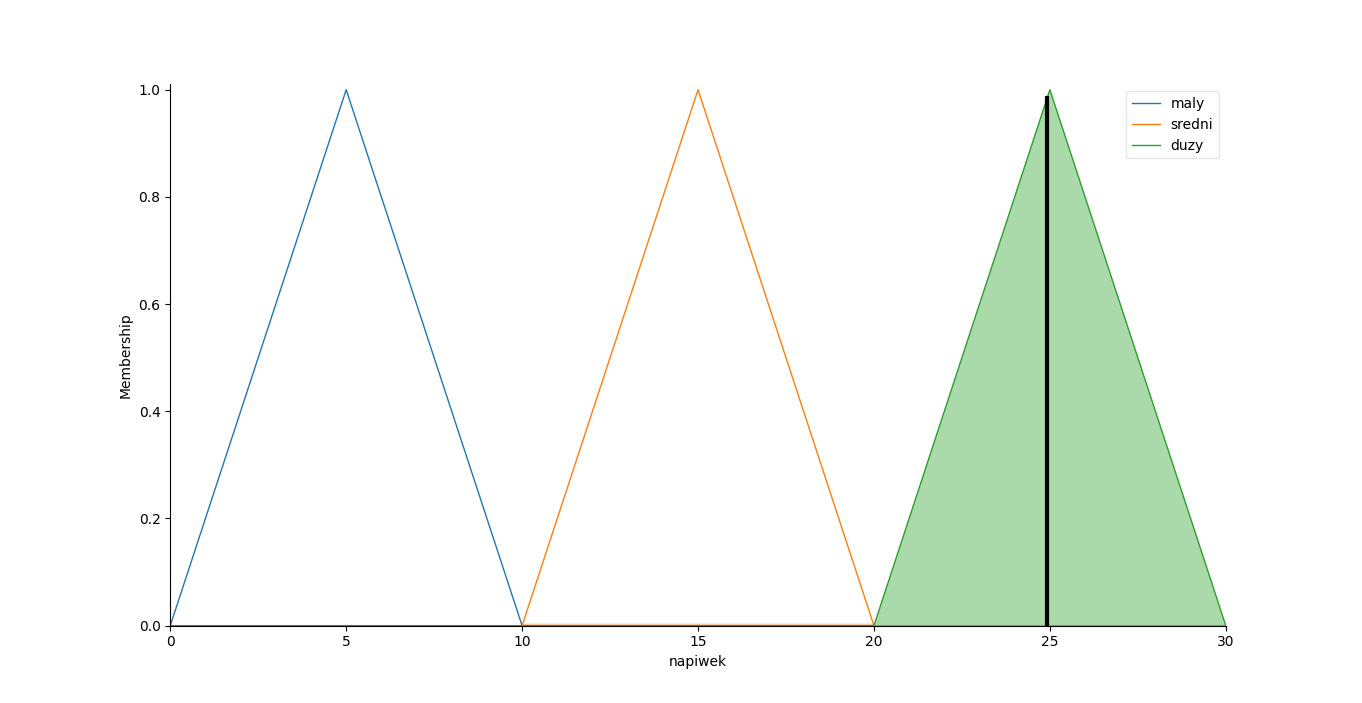
\includegraphics[scale=0.35]{Figure_4.png}
	\caption{\textit{Wyostrzenie metodą środka ciężkości dla wejścia obsługa = 10}}
	\label{fig:obsluga10}

\end{figure}

\subsubsection{Sprawdzenie działania systemu dla wartości obsługi}\label{ssc:sprawdzenie_dzialania_obsluga}

W tej sekcji sprawdzamy działanie systemu dla wartości obsługi od 0 do 10(rys. \ref{fig:napiwek_obsluga} wykres funkcji napiwek=f(obsluga)).

\lstinputlisting[style=PYTHON, firstline=41, lastline=53]{./code/main.py}

\begin{figure}[H]
	\centering
	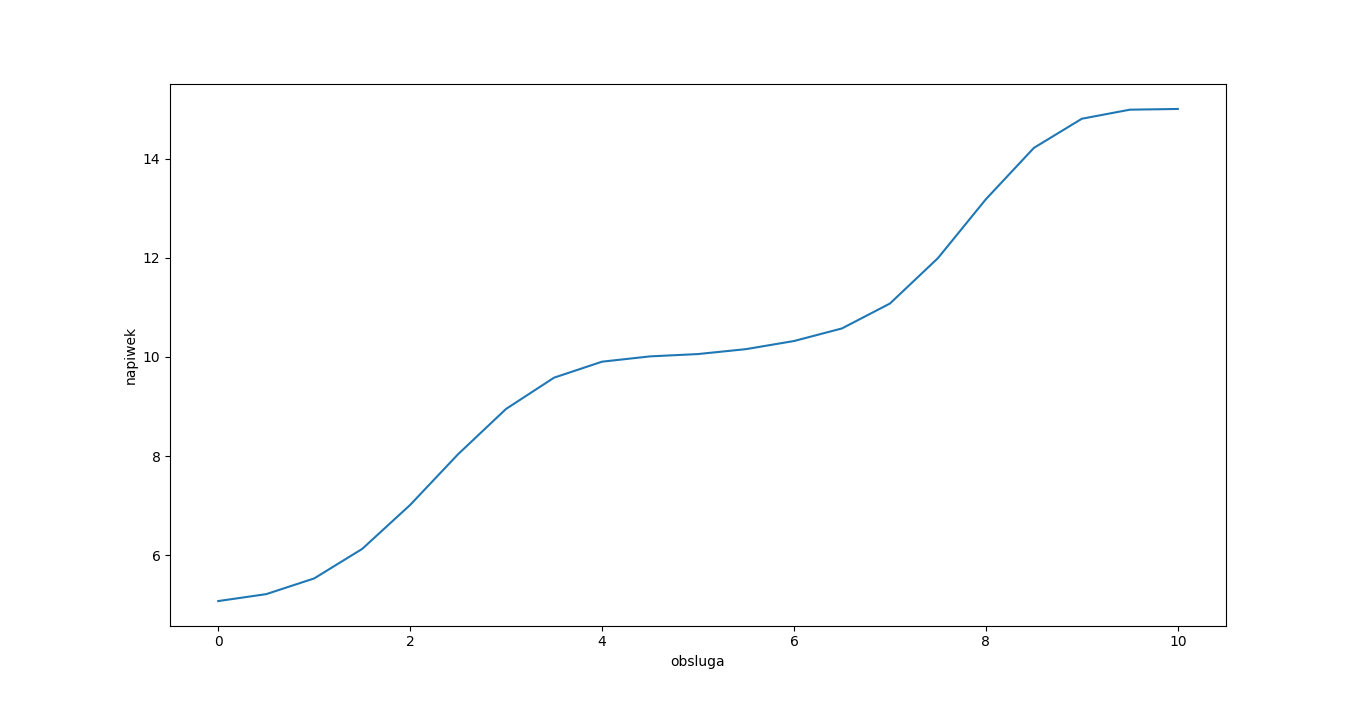
\includegraphics[scale=0.35]{Figure_5.png}
	\caption{\textit{Powierzchnia prejścia systemu ``napiwek'' o jednym wejściu}}
	\label{fig:napiwek_obsluga}
\end{figure}

\subsubsection{Dodanie drugiej wejściowej}\label{ssc:dodanie_wejsciowej}
 
W tej selcji dodajemy drugą wejściową zmienną stanu ``jedzenie'' o trapezoidalnych(\verb|trapmf|) zbiorach rozmytych ``zepsute'' oraz ``wyborne''.

\lstinputlisting[style=PYTHON, firstline=8, lastline=8]{./code/main.py}
\lstinputlisting[style=PYTHON, firstline=18, lastline=19]{./code/main.py}

\subsubsection{Dodanie reguł 4 i 5}\label{ssc:dodanie_regul45}

W tej sekcji dodajemy reguły 4 i 5 analogicznie do punktu \ref{ssc:definicja_regul}.

\lstinputlisting[style=PYTHON, firstline=28, lastline=29]{./code/main.py}

\subsubsection{Sprawdzenie działania systemu dla wartości ``obsługi''}\label{ssc:sprawdzenie_dzialania_wartosc_obsluga}

W tej sekcji sprawdzamy działanie systemu dla wartości obsługi równej \textbf{0} oraz wartości jedzenia równej \textbf{0}.

\lstinputlisting[style=PYTHON, firstline=34, lastline=39]{./code/main.py}

\subsubsection{Sprawdzenie działania systemu dla wartości ``obsługi'' i ``jedzenia''}\label{ssc:sprawdzenie_dzialania_obsluga_jedzenie}

W tej sekcji sprawdzamy działanie systemu dla wartości obsługi i jedzenia od 0 do 10(rys. \ref{fig:napiwek_obsluga_jedzenie})

\lstinputlisting[style=PYTHON, firstline=55,lastline=75]{./code/main.py}

\begin{figure}[h]
	\centering
	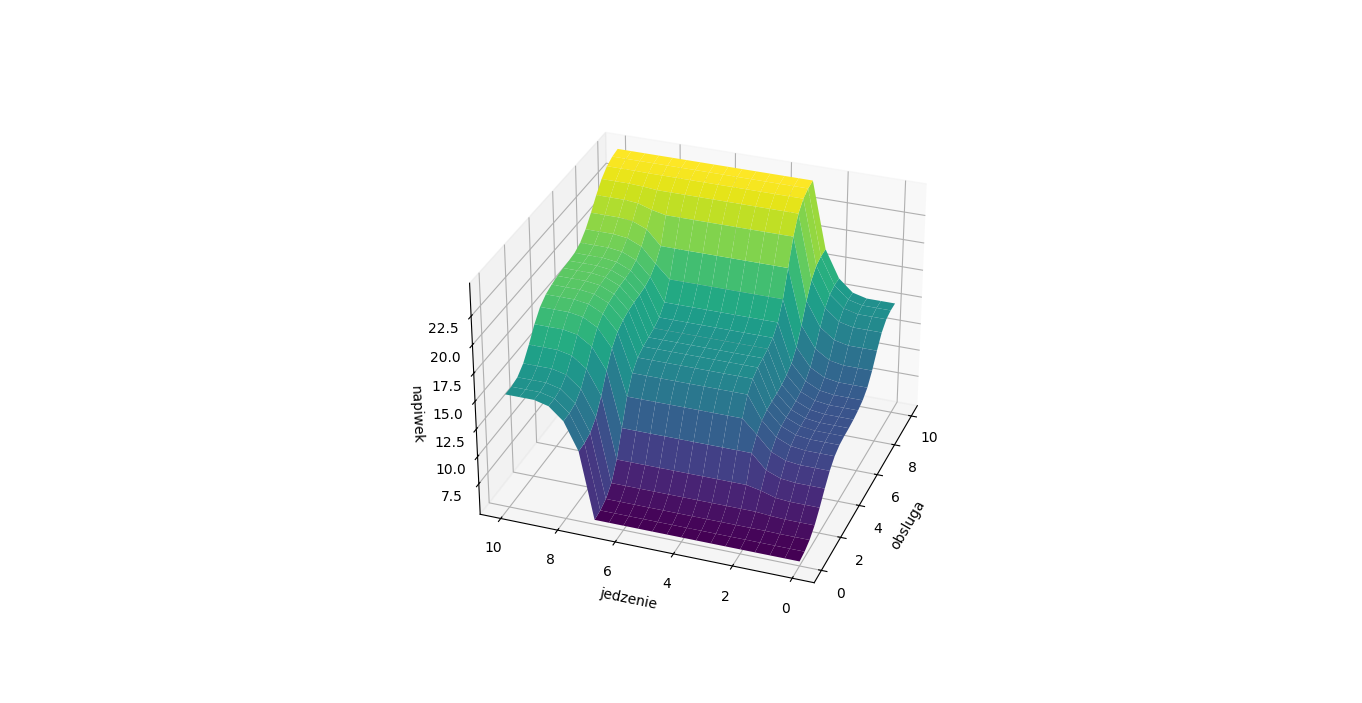
\includegraphics[scale=0.35]{Figure_7.png}
	\caption{\textit{Powierzchnia przejścia systemu ``napiwek'' o dwóch wejściach}}
	\label{fig:napiwek_obsluga_jedzenie}
\end{figure}

% modification section
\section{Modyfikacja systemu}\label{sec:modyfikacja}

% tasks section
\section{Przykładowe zadania zaliczeniowe}\label{sec:zadania}

% conclusion section
\section{Wnioski}\label{sec:wnioski}


\end{document}
